\chapter{Web Server - Design of Experiment}
Obiettivo: Design an experiment to study the impact of two factors (intensity and page type) on the response time
\section{Design}
Descrizione fattori scelti repliche ecc ...
collezionamento response time medio
\section{Analisi}
Il design oggetto di studio è un \textit{Two-factor Full Factorial Design con repliche}.
I fattori che lo interessano sono categorici, quindi possono assumere solo valori finiti. 
\\La seguente tabella descrive i tempi medi di risposta ottenuti in funzione delle combinazioni dei fattori e delle repliche:
\\
\begin{table*}[h]
	\begin{center}
		\begin{tabular}{|c|c|c|c|c|}
			\hline
			Intensity & Small & Small-Medium & Meduim-Large & Large\\
			\hline
			\rule[-4mm]{0mm}{0.5cm}
			1500 & 5,2082 & 23,5713 & 42,0207 & 78,6531\\
			\rule[-4mm]{0mm}{0.5cm}
			& 5,7017 & 16,3747 & 32,3323 & 54,5792\\
			\rule[-4mm]{0mm}{0.5cm}
			& 5,4777 & 19,1214 & 32,6010 & 39,0433\\
			\rule[-4mm]{0mm}{0.5cm}
			& 5,9955 & 14,0742 & 36,6634 & 47,6427\\	
			\rule[-4mm]{0mm}{0.5cm}
			& 5,1065 & 16,8909 & 41,6693 & 55,1706\\ 
			\hline
			\rule[-0.5cm]{0mm}{0.5cm}
			4500 & 5,1412 & 15,4733 & 380,9312 & 552,1893\\
			\rule[-0.5cm]{0mm}{0.5cm}
			& 4,5569 & 18,6695 & 379,4760 & 538,0078\\
			\rule[-0.5cm]{0mm}{0.5cm}
			& 4,6629 & 23,1843 & 375,8755 & 539,3999\\
			\rule[-0.5cm]{0mm}{0.5cm}
			& 4,4400 & 21,3396 & 366,9233 & 575,0426\\	
			\rule[-0.5cm]{0mm}{0.5cm}
			& 4,3709 & 20,0086 & 368,5614 & 541,5188\\
			\hline
		\end{tabular}
	\end{center}
\end{table*}
\\
\\
Vedere se aggiungere :
\\Equazione modello
\\Computation of Effects
\\Interactions
\\Computation of Errors
\\capire se l' f-value ha senso anche nel caso di test non parametrici
\subsection{Importanza - Allocation of Variation}
L' \textit{importanza} di un fattore viene misurata in base alla porzione di \textbf{variazione totale} che esso riesce a spiegare.
\\Quest'ultima è espressa tramite la Sum of Squares Total o \textit{SST} la quale ci fornisce informazioni circa quanto i dati ottenuti si discostano dal loro valore medio.
\begin{equation*}
	SST = \sum_{i = 1}^{n}{({y_i} - \overline{y})^2}
\end{equation*}
In particolare la variazione totale può essere anche vista come somma delle variazioni spiegate dai fattori, dalle loro interazioni e dall'errore commesso:
\\\textbf{SST = {SSA + SSB + SSAB + SSE}}.
\\La percentuale di variazione spiegata dal fattore A ad esempio è : \textbf{A = (SSA/SST)*100}.
\\
Queste informazioni possono essere agevolmente ottenute in \textit{JMP}, operando sulla tabella che caratterizza il design in questione, analizzando le sezioni:
\begin{enumerate}
	\item \textit{Analisi della varianza}
	\item \textit{Test degli effetti}
\end{enumerate}
\subsubsection{Caso di Studio}
\begin{figure}[H]
	\subfigure{	
		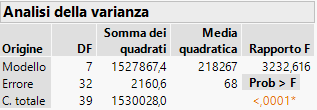
\includegraphics[width=0.50\textwidth]{img/hw4/AnalisiVarianza.png}}
	\subfigure{	
		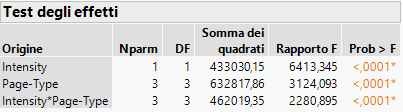
\includegraphics[width=0.50\textwidth]{img/hw4/TestEffetti.png}}
	\caption{\textit{Sum of Squares in JMP}}
\end{figure}
\begin{table*}[h]
	\begin{center}
		\begin{tabular}{|c|c|c|}
			\hline
			Component & Sum of Squares & \% Variation\\
			\hline
			 \rule[-4mm]{0mm}{0.5cm}
			 y - {$\overline{y}_...$}   	& 1530028,0		   & 100\\
			 \rule[-4mm]{0mm}{0.5cm}
			 Intensity (CTTs) 		  & 433030,15		   & 28,30\\
			 \rule[-4mm]{0mm}{0.5cm}
			 Page-Types 		  & 632817,86		   & 41,36\\
			 \rule[-4mm]{0mm}{0.5cm}
			 Interactions		  & 462019,35		   & 30,20\\
			 \rule[-4mm]{0mm}{0.5cm}
			 Errors 		  & 2160,6		   & 0,14\\
			\hline
		\end{tabular}
	\end{center}
\end{table*}
Osservando i risultati ottenuti notiamo che la percentuale maggiore di variazione la spiega il fattore \textit{Page Types}, con il 41,36\% della totale, seguito da \textit{Interazioni} e \textit{Intensità del carico} che ne spiegano una percentuale più o meno simile (rispettivamente 28,30\% e 30,20\%). Il restante 0,14\% è attribuita all'errore sperimentale.
\\
Tuttavia l'importanza non è un concetto statistico, dunque necessitiamo la valutazione di un altro parametro che invece lo è, la significatività.
Difatti può accadere che un fattore importante non sia significativo.
\subsection{Significatività - Analysis of Variance}
La \textit{significatività} di un fattore, come precedentemente specificato, è un concetto statistico il quale esplicita il contributo che spiega quel fattore rispetto a quello relativo all'errore.
\\Se un fattore è significativo, ripetendo l'esperimento, con elevata probabilità (associata al livello di significatività) esso influenzerà sempre allo stesso modo l'output, dimostrando che quindi quei risultati non sono dettati dal caso.
\\
\\Gli ANOVA (Analysis of Variance) tests permettono di verificare la significatività dei fattori di un esperimento. Al pari dei test d'ipotesi discussi nel capitolo precedente, anch'essi si basano su delle assunzioni tra cui:
\begin{itemize}
	\item \textbf{normalità dei residui}.
	\item \textbf{omoschedasticità}.
\end{itemize}
In base a se queste due condizioni sono verificate o meno, verrà utilizzato un particolare test. Nella seguente tabella sono sintetizzate tutte le combinazioni tra le varie condizioni con il relativo test da applicare:
\begin{figure}[H]
	\centering
	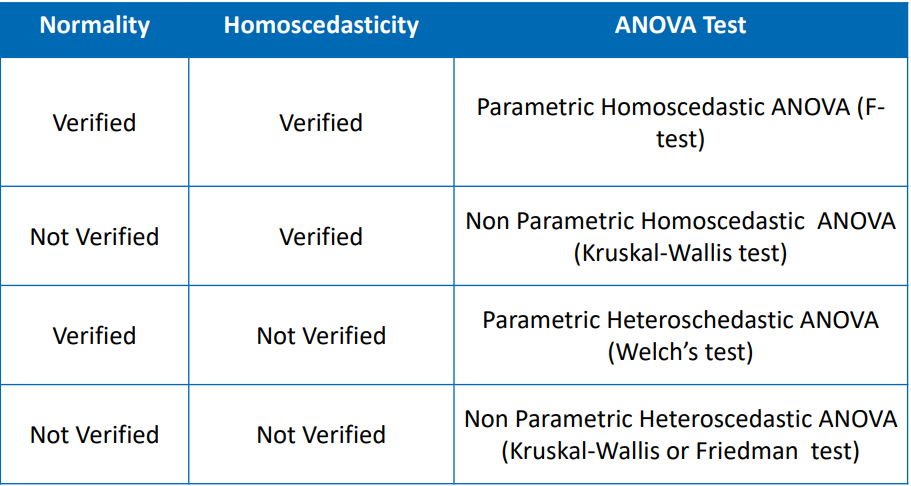
\includegraphics[width=0.8\textwidth]{img/hw4/ANOVATests.png}
	\caption{\textit{Tabella ANOVA tests}}
	\label{table}
\end{figure}
\subsubsection{Caso di Studio - Check Normalità}
Per poter decidere quale test utilizzare per studiare la significatività di \textit{Intensity} e \textit{Page-Types} dobbiamo quindi verificare innanzitutto se i residui (risposta osservata - valore previsto) provengono da una distribuzione normale.
\\JMP permette di ricavare la colonna dei residui automaticamente a partire da livelli - ripetizioni e output. Dopo averla generata ne plottiamo la distribuzione, in particolare il \textit{normal quantile plot}
\begin{figure}[H]
	\centering
	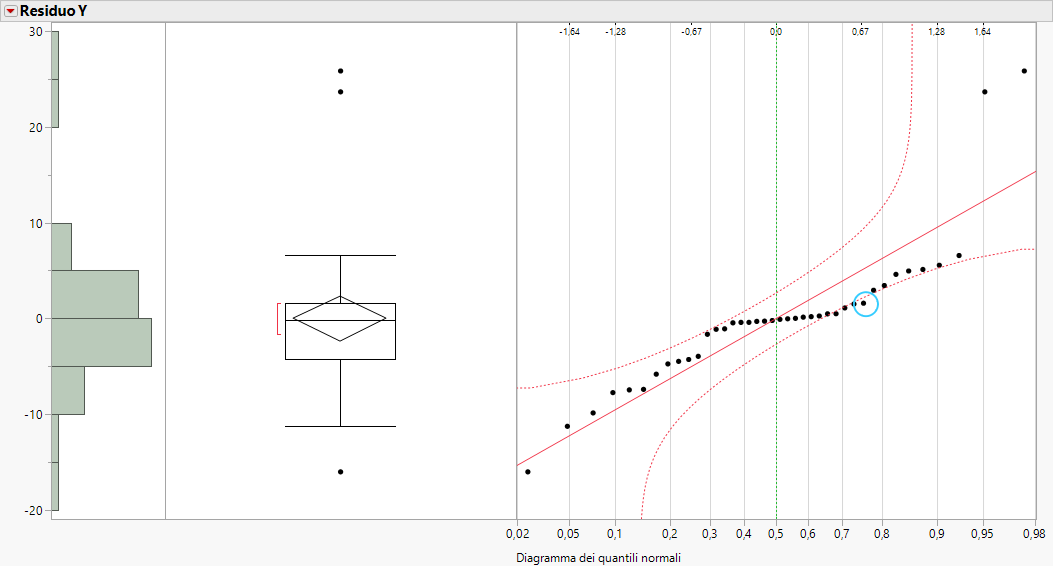
\includegraphics[width=0.8\textwidth]{img/hw4/qqplot_res.png}
	\caption{\textit{Normal quantile plot JMP}}
\end{figure}
il quale non è altro che il q-qplot già discusso per la workload characterization.
\\Assumiamo che la distribuzione considerata non è normale se anche uno solo dei residui esce al di fuori delle bande di confidenza (tratteggiate e in rosso). Nel nostro caso si verifica con evidenza proprio questa situazione, dunque \textbf{la normalità non è verificata}.
\\Potremmo validare ulteriormente tale assunzione attraverso il test statistico di \textit{Shapiro-Wilk}, tenendo conto del fatto che se dovesse fornire un risultato diverso da quello del test visivo, in ogni caso sarà l'esito di quest'ultimo (del test visivo) ad essere preferito.
\begin{figure}[H]
	\centering
	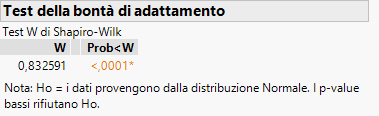
\includegraphics[width=0.5\textwidth]{img/hw4/shapiro_wilch.png}
	\caption{\textit{Test di Shapiro Wilk}}
\end{figure}
Il test ci restituisce un p-value basso, dunque l'ipotesi nulla è stata rigettata ad ulteriore conferma della non normalità della nostra distribuzione.
\subsubsection{Caso di Studio - Check Omoschedasticità}
L'uguaglianza delle varianze viene valutata esclusivamente per ogni fattore. Lo si fa prendendo in considerazione uno dei seguenti test:
\begin{enumerate}
	\item \textit{Bartlett}
	\item \textit{Levene}
	\item \textit{O'Brien}
	\item \textit{Brown-Forsythe}
\end{enumerate}
i cui risultati sono agevolmente forniti da JMP.
\begin{figure}[H]
	\subfigure{	
		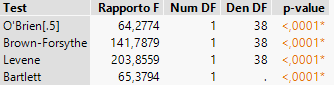
\includegraphics[width=0.50\textwidth]{img/hw4/omo_i.png}}
	\subfigure{	
		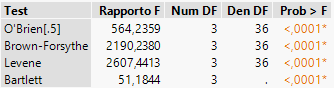
\includegraphics[width=0.50\textwidth]{img/hw4/omo_pt.png}}
	\caption{\textit{Test omoschedasticità Intensity e Page Type}}
\end{figure}
Indipendentemente dal test scelto, per entrambi i fattori \textbf{non vale l'ipotesi di omoschedasticità}. Difatti il p-value basso ci suggerisce che l'ipotesi nulla è stata rigettata.
\subsubsection{Caso di Studio - Check Significatività fattori}
Considerando la \ref{table} siamo nel caso 4, con normalità e omoschedasticità non verificate. I test da poter applicare fanno parte degli ANOVA non parametrici eteroschedastici: \textbf{Kruskal-Wallis test o Friedman test}.
Prendendo in considerazione il primo (sarebbe stato lo stesso anche se avessimo verificato l'omoschedasticità):
\begin{figure}[H]
	\centering
	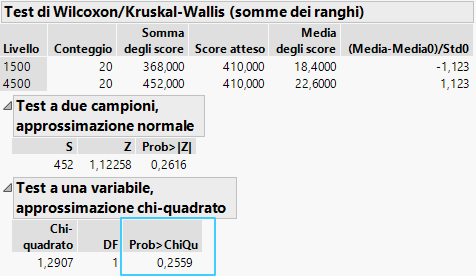
\includegraphics[width=0.6\textwidth]{img/hw4/KW_i.png}
	\caption{\textit{Test di Kruskal-Wallis Intensity}}
\end{figure}
Il valore alto (in nero) del p-value indica che il fattore Intensity non è risultato significativo ai fini dei tempi di risposta.
\begin{figure}[H]
	\centering
	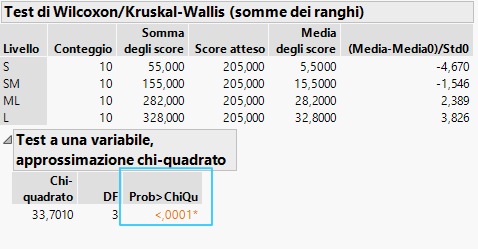
\includegraphics[width=0.6\textwidth]{img/hw4/KW_pt.png}
	\caption{\textit{Test di Kruskal-Wallis Page-Type}}
\end{figure}
Il p-value in questo caso assume un valore abbastanza piccolo (in arancione), dunque il fattore Page-Type oltre ad essere quello più importante risulta anche l'unico fattore significativo per l'output.
\\Ciò volendo ce lo aspettavamo perchè osservando i dati nella tabella del paragrafo analisi, diciamo che il tempo di risposta per pagine small e small-medium è lo stesso indipendentemente dal carico, non appena la dimensione, e quindi il tipo di pagina, aumenta/varia, i tempi di risposta associati ai due carichi sono completamente diversi. 